\chapter{実装}\label{sec:implementation}
本研究ではリファレンス実装として、C言語を中間表現とするSFRPのコンパイラ
\footnote{https://github.com/sfrp/sfrp}を作成した。
以降ではこの実装をSFRPコンパイラと呼称する。
本章では、SFRPコンパイラによってプログラムがどのように実行されるのかを説明する。

\section{SFRPプログラム例}\label{sec:implementation:example}
以降の節では、Code \ref{code:sample}に示す簡単なSFRPのプログラムBLINKLEDを例にとって解説および評価を行う。
このプログラムは、接続されたLEDの明滅を一定周期で切り替えるシステムを記述したものである。

マイクロコントローラには8KBのFlashと1KBのRAM、16MHzの内部クロックを持つAtmel AVR 8ビットマイクロコントローラ ATmega8
\footnote{http://www.atmel.com/ja/jp/devices/ATMEGA8.aspx}
を使用し、汎用入出力ポートPD7とGNDの間にLEDを接続する。
本来、I/O処理のインターフェースはアーキテクチャ毎に個別にユーザが定義する必要があるが、
本マイクロコントローラATmega8についてはリファレンス実装としてI/O処理がSFRPの標準ライブラリに組み込まれている。

\newpage
\lstinputlisting[language=SFRP,tabsize=2,caption={SFRPの例題プログラム(BLINKLED)},label={code:sample}]{./code/simple-example/BlinkLED.sfrp}


\section{実行過程}\label{sec:implementation:execution}
SFRPコンパイラによって、BLINKLEDは以下の繰り返し処理として実行される。
これは、\ref{sec:language:model:execution}項における実行モデルに基づいている。
\begin{figure}[h]
\begin{screen}
\begin{enumerate}
  \item 全ての初期値付きノードの初期値が計算され、初回の直前値として保持される。
    BLINKLEDの場合、初期値付きノードは\texttt{@led}のみである。
  \item 依存関係の順に従い、全てのノードの現在値が導出される。
    BLINKLEDの場合、入力ノードは存在せず、内部ノードも\texttt{@led}のみであるため、
    \texttt{@led}の現在値が計算されるのみである。
  \item ノード出力定義に従い、出力を行う。
    BLINKLEDの場合、13行目のノード出力定義に従い、
    \texttt{@led}の現在値がOnであるなら出力ポートPD7にTrue(High)が出力され、OffであるならFalse(Low)が出力される。
  \item 初期値付きノードの現在値は次回の計算フェーズまで保持され、次回の直前値として参照される。
    BLINKLEDの場合、\texttt{@led}の現在値が次回まで保持される。
  \item 2に戻る。
\end{enumerate}
\end{screen}
\caption{BLINKLEDの実行処理}
\label{fig:imp:exec}
\end{figure}

\section{式や関数の表現}\label{sec:implementation:expression}
SFRPの式や関数とC言語の式や関数の間にギャップはあまりないため、特に複雑な変換処理などは介さずにC言語へとコンパイルされる。
let式で導入される局所変数はその式が所属する関数の局所変数として巻き上げられ、パターンマッチ式やif式は3項演算子へと変換される。
関数呼び出しおよびコンストラクタ呼び出しはそのまま対応する関数の呼び出し式として表現される。
内部ノードは関数として表現され、依存する他のノードの参照は関数のパラメータを介して行われる。

\section{データ構造の確保と取り扱い}\label{sec:implementation:data}
SFRPコンパイラはデータ構造の実体を静的領域に確保し、実行時にはポインタを介してデータ構造を参照する。
ノードの現在値演算が一巡する毎(図\ref{fig:imp:exec}の第5項目を実行する毎)に全データ構造の参照到達性が調べられ、使用されていないデータ構造は再利用される。
このとき、初期値付きノードの現在値がルートとなって参照到達性の判定が行われる。

静的表域に確保するされるデータ構造の実体の必要数は図\ref{fig:memory-eval}の評価によって求めることができる。
BLINKLEDの場合、\texttt{Blink}型のデータ構造に対して必要な実体は2つである。


\section{実行時性能}\label{sec:implementation:performance}
本研究ではBLINKLEDの実行時性能を調査し、SFRP言語およびSFRPコンパイラの簡易的な実行性能評価とする。

\subsection{メモリ性能}
avr-gcc(v4.9.2)を用いてバイナリ(実行形式)を生成し、この実行形式を分析することによってメモリ使用量の算出を行う。
ただしコードサイズを小さくするため、以下のコンパイルオプションを指定した。
\begin{lstlisting}[basicstyle=\ttfamily\small,numbers=none,frame=none]
-Os -fdata-sections -ffunction-sections -Wl,--gc-sections
\end{lstlisting}
2つ目以降のオプションは不要な関数定義をバイナリに含めないようにするための指定である。

SFRPコンパイラが出力したC言語コードを元に関数コールグラフを作成すると図\ref{fig:imp:call_graph}に示す通りとなる。
ただし関数名の右横の数字はその関数で導入される局所変数のバイトサイズである。
このサイズはコンパイル時のgccにオプション\texttt{-fstack-usage}を指定することで求めることができる。
1回の関数呼び出しで消費するスタック領域を
\begin{center}
$スタックポインタを格納する2バイト領域 + 局所変数を格納する領域$
\end{center}
であると仮定すると、図\ref{fig:imp:call_graph}より最大スタック使用量は
\begin{center}
$(2 + 6) + (2 + 0) + (2 + 2) + (2 + 0) =$ 16 byte\\
\end{center}
であると算出される。

プログラムサイズおよび静的領域の使用量についてはavr-sizeコマンドによってそのまま求めることができる。
以上を纏めると表\ref{fig:imp:size}に示す通りとなり、
BLINKLEDのFlushの使用量は486byte、RAMの最大使用量は$8+16=$24byteであると算出される。

\begin{figure}[h]
 \begin{center}
  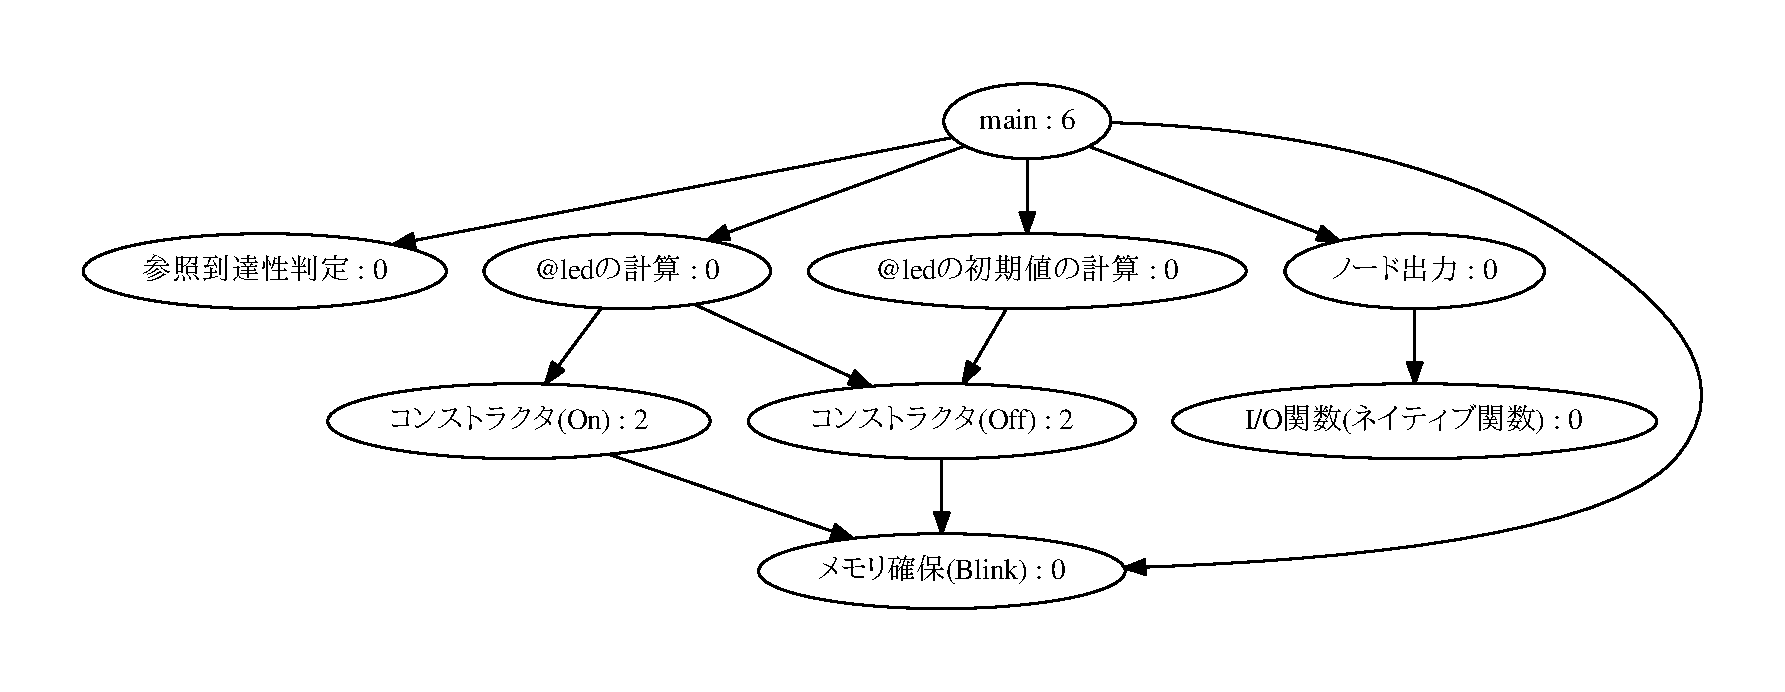
\includegraphics[width=160mm]{figure/call_graph.pdf}
 \end{center}
 \caption{BLINKLEDをコンパイルした結果の関数コールグラフ}
 \label{fig:imp:call_graph}
\end{figure}

\begin{table}[h]
  \centering
  \begin{tabular}{l|r}
    Programサイズ(avr-sizeコマンドより) & 486 byte \\ \hline
    Dataサイズ(avr-sizeコマンドより) & 8 byte \\ \hline
    最大スタックサイズ(-fstack-usageオプションおよび手計算により算出)  & 16 byte \\ \hline
  \end{tabular}
\caption{BLINKLEDのメモリ使用量}
\label{fig:imp:size}
\end{table}


\subsection{速度性能}\label{sec:implementation:performance:speed}
メモリ性能の評価と同じ条件で実行形式を生成し、ATmega8実機上で実際にプログラムを動かして実行速度を計測する。
実行速度はLEDの明滅切り替え(すなわち、出力のHigh/Lowの切り替え)の間隔を測定することによって求める。
この測定を、実時間計測が可能なもう1つのマイクロコントローラを接続することによって行ったところ、結果は表\ref{fig:imp:time1}の通りとなった。

\begin{table}[h]
  \centering
  \begin{tabular}{c}
    $ \input{code/simple-example/evaluation/result1.txt}ms$ \\ \hline
  \end{tabular}
\caption{BLINKLEDのLED明滅が切り替わる時間の間隔(20回平均)}
\label{fig:imp:time1}
\end{table}

プログラムBLINKLEDにおいて10000回のイテレーションを経てLEDの明滅が切り替わることから、
イテレーション1回(図\ref{fig:imp:exec}の一巡)に対して平均
$ \input{code/simple-example/evaluation/result2.txt} \mu s$
の計算時間を要していることがわかる。

イテレーション1回の計算に要する時間は当然プログラムに依存する。
しかしSFRP言語が再帰的関数の定義を認めていないことを考慮すれば、計算時間は概ねコードの分量に比例するであろうと予測できる。
従ってBLINKLEDよりも複雑でより実用的なプログラムを記述したとしても、イテレーション1回に要する時間はせいぜいこれの数倍から十数倍程度
(すなわち$1ms$から$10ms$程度)に収まるものと思われる。
この程度の所要時間であれば、多くの小規模組込みシステムにとっては十分な反応速度を得られるであろう。
